%Created with command:
%"/home/josh/Teaching/trunk/Utilities/makeexam" "Quiz 2" "Please show all work.  You may not use a calculator." "../VHDL/Assessments/interface_implementation.tex" "../CombinationalDesign/Assessments/timing_read_write.tex" "../Muxes/Assessments/74x138_demux.tex" "../VHDL/Assessments/eight_input_and_gate.tex"
\documentclass{article}
\usepackage[T1]{fontenc}
\usepackage{arev}
\usepackage{longtable}
\usepackage[hmargin=2cm,vmargin=2cm]{geometry}
\usepackage{graphicx}
\usepackage{listings}
\setlength{\parindent}{0pt}
\title{Quiz 2}
\date{}
\begin{document}
\maketitle
Please show all work.  You may not use a calculator. (12 points total)
\begin{longtable}[l]{rp{17cm}}
%file: ../VHDL/Assessments/interface_implementation.tex
1.&\begin{minipage}[t]{\linewidth}(2 pt) Explain how VHDL accomplishes the separation of interface from implementation (you probably only need to write one sentence, although you may write more).\\

Solution: \\ \\
VHDL entity statements provide an interface to a component, VHDL architecture statements provide the implementation of the component.
\end{minipage}\\
\medskip
%file: ../CombinationalDesign/Assessments/timing_read_write.tex
2.&\begin{minipage}[t]{\linewidth}(2 pt) You have been given the following timing diagram as part of the documentation for a circuit that you are reviewing.  Please explain a possible problem with the operation of this circuit.\\ \\
\begin{center}
  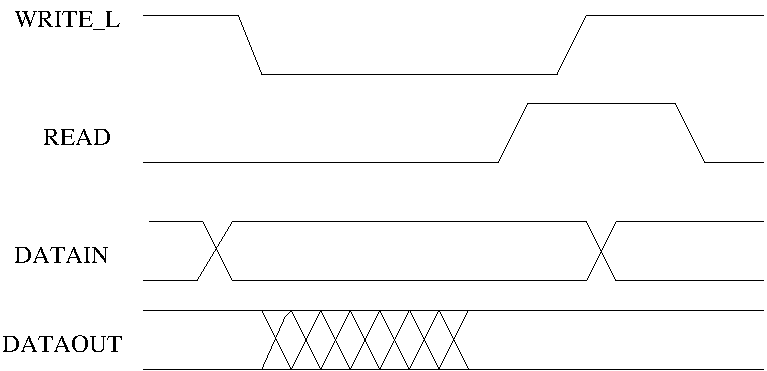
\includegraphics{../CombinationalDesign/Assessments/TimingDiagramReadWrite}
\end{center}

Solution: \\ \\
The data on DATAOUT will be read before it has been completely written.
\end{minipage}\\
\medskip
%file: ../Muxes/Assessments/74x138_demux.tex
3.&\begin{minipage}[t]{\linewidth}(4 pt) Using input signals SRC\_L, SEL0, SEL1, and SEL2, configure the inputs of the 74x128 decoder below to cause it to behave as a 1-bit demultiplexer.\\ \\
\begin{center}
  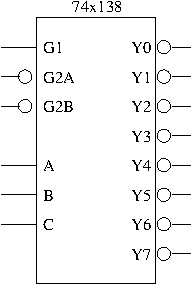
\includegraphics{../Muxes/Assessments/74x138Schematic}
\end{center}

Solution: \\ \\
\begin{center}
  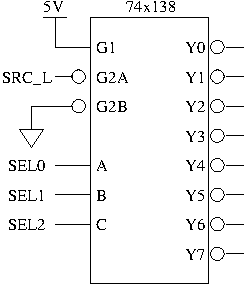
\includegraphics{../Muxes/Assessments/74x138DMuxSchematic}
\end{center}
\end{minipage}\\
\medskip
%file: ../VHDL/Assessments/eight_input_and_gate.tex
4.&\begin{minipage}[t]{\linewidth}(4 pt) Using VHDL, write the architecture for an eight input AND gate.  Use the entity provided below.  I will email you a test bench that you should use to validate your program.  You may use your text, examples from class, and even resources on from the Internet for this problem.  However, please \textbf{do not dicuss the solution to this problem with other students in this class}.\\
\lstset{language=VHDL}
\begin{lstlisting}
entity eight_input_and_gate is
    port (X: in std_logic_vector(7 downto 0);
          F: out std_logic);
end eight_input_and_gate;
\end{lstlisting}

Solution: \\ \\
\lstinputlisting{../VHDL/Assessments/eight_input_and_gate.vhd}
\end{minipage}\\
\medskip
\end{longtable}
\end{document}